% =====================================================================
%  4EK453 Principy ekonometrie – pokyny k semestrální práci
%  Vychází z pokynů 4EK216 (semestralni_prace.tex, 2018) a dodatku
%  „Časté chyby v semestrálních pracích“ (ChybySemestrálka.docx, 2022).
%  Překlad (ve složce semestralka/): xelatex 4EK453_semestralni_prace.tex (2×)
% =====================================================================
\documentclass[11pt,a4paper]{article}
% =====================================================================
%  Společná preambule textových dokumentů 4EK453 (A4): příklady ke cvičení
%  (cviceni/) a otázky ke zkoušce (zkouska/). Vkládá se za \documentclass:
%    \documentclass[11pt,a4paper]{article}
%    % =====================================================================
%  Společná preambule textových dokumentů 4EK453 (A4): příklady ke cvičení
%  (cviceni/) a otázky ke zkoušce (zkouska/). Vkládá se za \documentclass:
%    \documentclass[11pt,a4paper]{article}
%    % =====================================================================
%  Společná preambule textových dokumentů 4EK453 (A4): příklady ke cvičení
%  (cviceni/) a otázky ke zkoušce (zkouska/). Vkládá se za \documentclass:
%    \documentclass[11pt,a4paper]{article}
%    \input{../prezentace/src/_shared/dokument.tex}
%  Překlad: xelatex (2×). Značení a makra jsou stejná jako v prezentacích
%  (makra.tex), barvy stejné jako v beamerthemeFIS.sty.
% =====================================================================

% Pořadí: babel a mathtools před unicode-math (jinak kolize aktivního znaku „-“
% a mathtools přepíše \underbrace verzí pro staré fonty)
\usepackage[czech]{babel}
\usepackage{amsmath}
\usepackage{mathtools}
% Písma: Latin Modern, volaná jménem souboru (jako v _quarto.yml)
\usepackage{fontspec}
\usepackage{unicode-math}
\setmainfont{lmroman10}[Extension=.otf, UprightFont=*-regular, BoldFont=*-bold,
  ItalicFont=*-italic, BoldItalicFont=*-bolditalic]
\setsansfont{lmsans10}[Extension=.otf, UprightFont=*-regular, BoldFont=*-bold,
  ItalicFont=*-oblique, BoldItalicFont=*-boldoblique]
\setmonofont{lmmono10}[Extension=.otf, UprightFont=*-regular, ItalicFont=*-italic]
\setmathfont{latinmodern-math.otf}

\AtBeginDocument{\shorthandoff{-"}}

\usepackage[a4paper, left=25mm, right=25mm, top=25mm, bottom=25mm, headsep=8mm]{geometry}
\usepackage{xcolor}
\usepackage{booktabs}
\usepackage{array}
\usepackage{enumitem}
\usepackage{comment}
\usepackage{fancyvrb}
\usepackage{titlesec}
\usepackage{fancyhdr}
\usepackage{etoolbox}
\usepackage[hidelinks]{hyperref}

% Barvy FIS VŠE (stejné jako v beamerthemeFIS.sty)
\definecolor{fisZelena}{HTML}{00957D}
\definecolor{fisZelenaTmava}{HTML}{006E5C}
\definecolor{fisZelenaSvetla}{HTML}{DFF1EC}
\definecolor{fisSeda}{HTML}{54585A}
\definecolor{fisSedaSvetla}{HTML}{7C8183}
\definecolor{fisLinka}{HTML}{DCE0DF}
\definecolor{fisPodklad}{HTML}{EBF0EE}
\definecolor{fisCerna}{HTML}{1D1F20}
\definecolor{fisModra}{HTML}{0072B0}
\definecolor{fisCervena}{HTML}{D0453A}

% cesta ke sdíleným souborům; dokument hlouběji ve stromu si ji nastaví před \input,
% např. \newcommand{\sdilene}{../../prezentace/src/_shared/}
\providecommand{\sdilene}{../prezentace/src/_shared/}
% název kurzu v~titulku a záhlaví; dokument pro více kurzů (MP) si před \input
% nastaví \def\kurz{} a řádek s~kurzem se nevysází
\providecommand{\kurz}{4EK453 Principy ekonometrie}
\input{\sdilene makra.tex}

% ---------------------------------------------------------------------
%  Sazba
% ---------------------------------------------------------------------
\setlength{\parindent}{0pt}
\setlength{\parskip}{4pt plus 1pt}
\renewcommand{\arraystretch}{1.1}
\frenchspacing
\setlength{\emergencystretch}{2em}% dlouhé \texttt{…} a vzorce raději řídčeji než přes okraj

\titleformat{\section}{\sffamily\Large\bfseries\color{fisZelenaTmava}}{\thesection}{0.6em}{}
\titleformat{\subsection}{\sffamily\large\bfseries\color{fisSeda}}{\thesubsection}{0.6em}{}
\titlespacing*{\section}{0pt}{16pt plus 4pt}{6pt}
\titlespacing*{\subsection}{0pt}{12pt plus 3pt}{4pt}
\renewcommand{\paragraph}[1]{\par\medskip\noindent{\sffamily\bfseries\color{fisZelenaTmava}#1}\quad}

% Titulek: \title, \subtitle, \author, \institution; datum = datum překladu (verze)
\makeatletter
\newcommand{\subtitle}[1]{\gdef\@subtitle{#1}}
\newcommand{\institution}[1]{\gdef\@institution{#1}}
\gdef\@subtitle{}\gdef\@institution{}
\renewcommand{\maketitle}{%
  \thispagestyle{plain}%
  {\color{fisZelena}\rule{\linewidth}{2pt}}\par\vspace{4pt}%
  \ifx\kurz\@empty\else{\sffamily\small\color{fisSeda}\kurz\par}\vspace{2pt}\fi
  {\sffamily\LARGE\bfseries\color{fisCerna}\@title\par}\vspace{2pt}%
  \ifx\@subtitle\@empty\else{\sffamily\large\color{fisSeda}\@subtitle\par}\fi
  \vspace{6pt}%
  {\small\@author\ \textbar\ \@institution\hfill verze z~\@date\par}%
  \vspace{2pt}{\color{fisZelena}\rule{\linewidth}{0.6pt}}\par\vspace{8pt}}
\makeatother
\date{\today}

\pagestyle{fancy}
\fancyhf{}
\renewcommand{\headrulewidth}{0.4pt}
\renewcommand{\headrule}{{\color{fisLinka}\hrule height\headrulewidth}}
\makeatletter
\fancyhead[L]{\sffamily\footnotesize\color{fisSeda}\kurz}
\fancyhead[R]{\sffamily\footnotesize\color{fisSeda}\@title\ \textbar\ \@date}
\makeatother
\fancyfoot[C]{\sffamily\footnotesize\color{fisSeda}\thepage}
\fancypagestyle{plain}{\fancyhf{}\renewcommand{\headrulewidth}{0pt}%
  \fancyfoot[C]{\sffamily\footnotesize\color{fisSeda}\thepage}}

% ---------------------------------------------------------------------
%  Příklady
% ---------------------------------------------------------------------
% \begin{priklad} … \end{priklad}         úloha na papír
% \begin{priklad}[R] … \end{priklad}      úloha na počítači (v R)
% \koumaci                                označení „(Pro koumáky.)“
% \begin{prikladlist} \item … \end{prikladlist}   podúlohy a), b), …
% \begin{reseni} … \end{reseni}           řešení; tisk řídí \includecomment / \excludecomment
\newcounter{priklad}[section]
\renewcommand{\thepriklad}{\ifnum\value{section}>0 \thesection.\fi\arabic{priklad}}
% značka R: malý obdélník bez \strut, spodkem barvy na účaří (nezvětšuje výšku řádku)
\newcommand{\znackaR}{\,{\setlength{\fboxsep}{1.3pt}\raisebox{\fboxsep}{\colorbox{fisZelena}{\sffamily\scriptsize\bfseries\color{white}\,R\,}}}}
% (Pro koumáky.) = vyžaduje aparát, který studenti nemusí mít (integrály, Choleského
% rozklad, obtížnější důkazy); u podúloh je dáváme na konec příkladu
\newcommand{\koumaci}{(\textit{Pro koumáky.})\ }% závorky stojatě
\NewDocumentEnvironment{priklad}{o}{%
  \par\addvspace{8pt}\refstepcounter{priklad}%
  \noindent{\sffamily\bfseries\color{fisZelenaTmava}Příklad~\thepriklad}%
  \IfValueT{#1}{\hspace{0.3em}\znackaR}\quad\ignorespaces}{\par\addvspace{4pt}}
\newlist{prikladlist}{enumerate}{1}
\setlist[prikladlist]{label=\textsl{\alph*})~, leftmargin=2em, itemsep=1pt, topsep=2pt}
\newcommand{\rada}{\par\smallskip\textit{Rada:} }
\newcommand{\pozn}{\par\smallskip\textit{Poznámka:} }

% Číslovaný seznam otázek s předponou (T1, T2, … / P1, P2, …), číslování
% pokračuje přes nadpisy: \begin{otazky}{T} … \end{otazky}
\newlist{otazkyT}{enumerate}{1}
\setlist[otazkyT]{label=\textbf{\sffamily\color{fisZelenaTmava}T\arabic*.}, ref=T\arabic*, resume,
  leftmargin=3em, itemsep=3pt, topsep=3pt}
\newlist{otazkyP}{enumerate}{1}
\setlist[otazkyP]{label=\textbf{\sffamily\color{fisZelenaTmava}P\arabic*.}, ref=P\arabic*, resume,
  leftmargin=3em, itemsep=6pt, topsep=3pt}

% Výpisy z R (vstupují ze souborů vygenerovaných skriptem, nikdy ne opsané ručně)
\fvset{fontsize=\small, xleftmargin=0.5em, frame=leftline, rulecolor=\color{fisLinka},
  framerule=1.5pt, framesep=5pt}
% výpis se nedělí mezi stránky
\newcommand{\vystupR}[1]{\par\noindent\begin{minipage}{\linewidth}\VerbatimInput{#1}\end{minipage}\par}

%  Překlad: xelatex (2×). Značení a makra jsou stejná jako v prezentacích
%  (makra.tex), barvy stejné jako v beamerthemeFIS.sty.
% =====================================================================

% Pořadí: babel a mathtools před unicode-math (jinak kolize aktivního znaku „-“
% a mathtools přepíše \underbrace verzí pro staré fonty)
\usepackage[czech]{babel}
\usepackage{amsmath}
\usepackage{mathtools}
% Písma: Latin Modern, volaná jménem souboru (jako v _quarto.yml)
\usepackage{fontspec}
\usepackage{unicode-math}
\setmainfont{lmroman10}[Extension=.otf, UprightFont=*-regular, BoldFont=*-bold,
  ItalicFont=*-italic, BoldItalicFont=*-bolditalic]
\setsansfont{lmsans10}[Extension=.otf, UprightFont=*-regular, BoldFont=*-bold,
  ItalicFont=*-oblique, BoldItalicFont=*-boldoblique]
\setmonofont{lmmono10}[Extension=.otf, UprightFont=*-regular, ItalicFont=*-italic]
\setmathfont{latinmodern-math.otf}

\AtBeginDocument{\shorthandoff{-"}}

\usepackage[a4paper, left=25mm, right=25mm, top=25mm, bottom=25mm, headsep=8mm]{geometry}
\usepackage{xcolor}
\usepackage{booktabs}
\usepackage{array}
\usepackage{enumitem}
\usepackage{comment}
\usepackage{fancyvrb}
\usepackage{titlesec}
\usepackage{fancyhdr}
\usepackage{etoolbox}
\usepackage[hidelinks]{hyperref}

% Barvy FIS VŠE (stejné jako v beamerthemeFIS.sty)
\definecolor{fisZelena}{HTML}{00957D}
\definecolor{fisZelenaTmava}{HTML}{006E5C}
\definecolor{fisZelenaSvetla}{HTML}{DFF1EC}
\definecolor{fisSeda}{HTML}{54585A}
\definecolor{fisSedaSvetla}{HTML}{7C8183}
\definecolor{fisLinka}{HTML}{DCE0DF}
\definecolor{fisPodklad}{HTML}{EBF0EE}
\definecolor{fisCerna}{HTML}{1D1F20}
\definecolor{fisModra}{HTML}{0072B0}
\definecolor{fisCervena}{HTML}{D0453A}

% cesta ke sdíleným souborům; dokument hlouběji ve stromu si ji nastaví před \input,
% např. \newcommand{\sdilene}{../../prezentace/src/_shared/}
\providecommand{\sdilene}{../prezentace/src/_shared/}
% název kurzu v~titulku a záhlaví; dokument pro více kurzů (MP) si před \input
% nastaví \def\kurz{} a řádek s~kurzem se nevysází
\providecommand{\kurz}{4EK453 Principy ekonometrie}
\input{\sdilene makra.tex}

% ---------------------------------------------------------------------
%  Sazba
% ---------------------------------------------------------------------
\setlength{\parindent}{0pt}
\setlength{\parskip}{4pt plus 1pt}
\renewcommand{\arraystretch}{1.1}
\frenchspacing
\setlength{\emergencystretch}{2em}% dlouhé \texttt{…} a vzorce raději řídčeji než přes okraj

\titleformat{\section}{\sffamily\Large\bfseries\color{fisZelenaTmava}}{\thesection}{0.6em}{}
\titleformat{\subsection}{\sffamily\large\bfseries\color{fisSeda}}{\thesubsection}{0.6em}{}
\titlespacing*{\section}{0pt}{16pt plus 4pt}{6pt}
\titlespacing*{\subsection}{0pt}{12pt plus 3pt}{4pt}
\renewcommand{\paragraph}[1]{\par\medskip\noindent{\sffamily\bfseries\color{fisZelenaTmava}#1}\quad}

% Titulek: \title, \subtitle, \author, \institution; datum = datum překladu (verze)
\makeatletter
\newcommand{\subtitle}[1]{\gdef\@subtitle{#1}}
\newcommand{\institution}[1]{\gdef\@institution{#1}}
\gdef\@subtitle{}\gdef\@institution{}
\renewcommand{\maketitle}{%
  \thispagestyle{plain}%
  {\color{fisZelena}\rule{\linewidth}{2pt}}\par\vspace{4pt}%
  \ifx\kurz\@empty\else{\sffamily\small\color{fisSeda}\kurz\par}\vspace{2pt}\fi
  {\sffamily\LARGE\bfseries\color{fisCerna}\@title\par}\vspace{2pt}%
  \ifx\@subtitle\@empty\else{\sffamily\large\color{fisSeda}\@subtitle\par}\fi
  \vspace{6pt}%
  {\small\@author\ \textbar\ \@institution\hfill verze z~\@date\par}%
  \vspace{2pt}{\color{fisZelena}\rule{\linewidth}{0.6pt}}\par\vspace{8pt}}
\makeatother
\date{\today}

\pagestyle{fancy}
\fancyhf{}
\renewcommand{\headrulewidth}{0.4pt}
\renewcommand{\headrule}{{\color{fisLinka}\hrule height\headrulewidth}}
\makeatletter
\fancyhead[L]{\sffamily\footnotesize\color{fisSeda}\kurz}
\fancyhead[R]{\sffamily\footnotesize\color{fisSeda}\@title\ \textbar\ \@date}
\makeatother
\fancyfoot[C]{\sffamily\footnotesize\color{fisSeda}\thepage}
\fancypagestyle{plain}{\fancyhf{}\renewcommand{\headrulewidth}{0pt}%
  \fancyfoot[C]{\sffamily\footnotesize\color{fisSeda}\thepage}}

% ---------------------------------------------------------------------
%  Příklady
% ---------------------------------------------------------------------
% \begin{priklad} … \end{priklad}         úloha na papír
% \begin{priklad}[R] … \end{priklad}      úloha na počítači (v R)
% \koumaci                                označení „(Pro koumáky.)“
% \begin{prikladlist} \item … \end{prikladlist}   podúlohy a), b), …
% \begin{reseni} … \end{reseni}           řešení; tisk řídí \includecomment / \excludecomment
\newcounter{priklad}[section]
\renewcommand{\thepriklad}{\ifnum\value{section}>0 \thesection.\fi\arabic{priklad}}
% značka R: malý obdélník bez \strut, spodkem barvy na účaří (nezvětšuje výšku řádku)
\newcommand{\znackaR}{\,{\setlength{\fboxsep}{1.3pt}\raisebox{\fboxsep}{\colorbox{fisZelena}{\sffamily\scriptsize\bfseries\color{white}\,R\,}}}}
% (Pro koumáky.) = vyžaduje aparát, který studenti nemusí mít (integrály, Choleského
% rozklad, obtížnější důkazy); u podúloh je dáváme na konec příkladu
\newcommand{\koumaci}{(\textit{Pro koumáky.})\ }% závorky stojatě
\NewDocumentEnvironment{priklad}{o}{%
  \par\addvspace{8pt}\refstepcounter{priklad}%
  \noindent{\sffamily\bfseries\color{fisZelenaTmava}Příklad~\thepriklad}%
  \IfValueT{#1}{\hspace{0.3em}\znackaR}\quad\ignorespaces}{\par\addvspace{4pt}}
\newlist{prikladlist}{enumerate}{1}
\setlist[prikladlist]{label=\textsl{\alph*})~, leftmargin=2em, itemsep=1pt, topsep=2pt}
\newcommand{\rada}{\par\smallskip\textit{Rada:} }
\newcommand{\pozn}{\par\smallskip\textit{Poznámka:} }

% Číslovaný seznam otázek s předponou (T1, T2, … / P1, P2, …), číslování
% pokračuje přes nadpisy: \begin{otazky}{T} … \end{otazky}
\newlist{otazkyT}{enumerate}{1}
\setlist[otazkyT]{label=\textbf{\sffamily\color{fisZelenaTmava}T\arabic*.}, ref=T\arabic*, resume,
  leftmargin=3em, itemsep=3pt, topsep=3pt}
\newlist{otazkyP}{enumerate}{1}
\setlist[otazkyP]{label=\textbf{\sffamily\color{fisZelenaTmava}P\arabic*.}, ref=P\arabic*, resume,
  leftmargin=3em, itemsep=6pt, topsep=3pt}

% Výpisy z R (vstupují ze souborů vygenerovaných skriptem, nikdy ne opsané ručně)
\fvset{fontsize=\small, xleftmargin=0.5em, frame=leftline, rulecolor=\color{fisLinka},
  framerule=1.5pt, framesep=5pt}
% výpis se nedělí mezi stránky
\newcommand{\vystupR}[1]{\par\noindent\begin{minipage}{\linewidth}\VerbatimInput{#1}\end{minipage}\par}

%  Překlad: xelatex (2×). Značení a makra jsou stejná jako v prezentacích
%  (makra.tex), barvy stejné jako v beamerthemeFIS.sty.
% =====================================================================

% Pořadí: babel a mathtools před unicode-math (jinak kolize aktivního znaku „-“
% a mathtools přepíše \underbrace verzí pro staré fonty)
\usepackage[czech]{babel}
\usepackage{amsmath}
\usepackage{mathtools}
% Písma: Latin Modern, volaná jménem souboru (jako v _quarto.yml)
\usepackage{fontspec}
\usepackage{unicode-math}
\setmainfont{lmroman10}[Extension=.otf, UprightFont=*-regular, BoldFont=*-bold,
  ItalicFont=*-italic, BoldItalicFont=*-bolditalic]
\setsansfont{lmsans10}[Extension=.otf, UprightFont=*-regular, BoldFont=*-bold,
  ItalicFont=*-oblique, BoldItalicFont=*-boldoblique]
\setmonofont{lmmono10}[Extension=.otf, UprightFont=*-regular, ItalicFont=*-italic]
\setmathfont{latinmodern-math.otf}

\AtBeginDocument{\shorthandoff{-"}}

\usepackage[a4paper, left=25mm, right=25mm, top=25mm, bottom=25mm, headsep=8mm]{geometry}
\usepackage{xcolor}
\usepackage{booktabs}
\usepackage{array}
\usepackage{enumitem}
\usepackage{comment}
\usepackage{fancyvrb}
\usepackage{titlesec}
\usepackage{fancyhdr}
\usepackage{etoolbox}
\usepackage[hidelinks]{hyperref}

% Barvy FIS VŠE (stejné jako v beamerthemeFIS.sty)
\definecolor{fisZelena}{HTML}{00957D}
\definecolor{fisZelenaTmava}{HTML}{006E5C}
\definecolor{fisZelenaSvetla}{HTML}{DFF1EC}
\definecolor{fisSeda}{HTML}{54585A}
\definecolor{fisSedaSvetla}{HTML}{7C8183}
\definecolor{fisLinka}{HTML}{DCE0DF}
\definecolor{fisPodklad}{HTML}{EBF0EE}
\definecolor{fisCerna}{HTML}{1D1F20}
\definecolor{fisModra}{HTML}{0072B0}
\definecolor{fisCervena}{HTML}{D0453A}

% cesta ke sdíleným souborům; dokument hlouběji ve stromu si ji nastaví před \input,
% např. \newcommand{\sdilene}{../../prezentace/src/_shared/}
\providecommand{\sdilene}{../prezentace/src/_shared/}
% název kurzu v~titulku a záhlaví; dokument pro více kurzů (MP) si před \input
% nastaví \def\kurz{} a řádek s~kurzem se nevysází
\providecommand{\kurz}{4EK453 Principy ekonometrie}
\input{\sdilene makra.tex}

% ---------------------------------------------------------------------
%  Sazba
% ---------------------------------------------------------------------
\setlength{\parindent}{0pt}
\setlength{\parskip}{4pt plus 1pt}
\renewcommand{\arraystretch}{1.1}
\frenchspacing
\setlength{\emergencystretch}{2em}% dlouhé \texttt{…} a vzorce raději řídčeji než přes okraj

\titleformat{\section}{\sffamily\Large\bfseries\color{fisZelenaTmava}}{\thesection}{0.6em}{}
\titleformat{\subsection}{\sffamily\large\bfseries\color{fisSeda}}{\thesubsection}{0.6em}{}
\titlespacing*{\section}{0pt}{16pt plus 4pt}{6pt}
\titlespacing*{\subsection}{0pt}{12pt plus 3pt}{4pt}
\renewcommand{\paragraph}[1]{\par\medskip\noindent{\sffamily\bfseries\color{fisZelenaTmava}#1}\quad}

% Titulek: \title, \subtitle, \author, \institution; datum = datum překladu (verze)
\makeatletter
\newcommand{\subtitle}[1]{\gdef\@subtitle{#1}}
\newcommand{\institution}[1]{\gdef\@institution{#1}}
\gdef\@subtitle{}\gdef\@institution{}
\renewcommand{\maketitle}{%
  \thispagestyle{plain}%
  {\color{fisZelena}\rule{\linewidth}{2pt}}\par\vspace{4pt}%
  \ifx\kurz\@empty\else{\sffamily\small\color{fisSeda}\kurz\par}\vspace{2pt}\fi
  {\sffamily\LARGE\bfseries\color{fisCerna}\@title\par}\vspace{2pt}%
  \ifx\@subtitle\@empty\else{\sffamily\large\color{fisSeda}\@subtitle\par}\fi
  \vspace{6pt}%
  {\small\@author\ \textbar\ \@institution\hfill verze z~\@date\par}%
  \vspace{2pt}{\color{fisZelena}\rule{\linewidth}{0.6pt}}\par\vspace{8pt}}
\makeatother
\date{\today}

\pagestyle{fancy}
\fancyhf{}
\renewcommand{\headrulewidth}{0.4pt}
\renewcommand{\headrule}{{\color{fisLinka}\hrule height\headrulewidth}}
\makeatletter
\fancyhead[L]{\sffamily\footnotesize\color{fisSeda}\kurz}
\fancyhead[R]{\sffamily\footnotesize\color{fisSeda}\@title\ \textbar\ \@date}
\makeatother
\fancyfoot[C]{\sffamily\footnotesize\color{fisSeda}\thepage}
\fancypagestyle{plain}{\fancyhf{}\renewcommand{\headrulewidth}{0pt}%
  \fancyfoot[C]{\sffamily\footnotesize\color{fisSeda}\thepage}}

% ---------------------------------------------------------------------
%  Příklady
% ---------------------------------------------------------------------
% \begin{priklad} … \end{priklad}         úloha na papír
% \begin{priklad}[R] … \end{priklad}      úloha na počítači (v R)
% \koumaci                                označení „(Pro koumáky.)“
% \begin{prikladlist} \item … \end{prikladlist}   podúlohy a), b), …
% \begin{reseni} … \end{reseni}           řešení; tisk řídí \includecomment / \excludecomment
\newcounter{priklad}[section]
\renewcommand{\thepriklad}{\ifnum\value{section}>0 \thesection.\fi\arabic{priklad}}
% značka R: malý obdélník bez \strut, spodkem barvy na účaří (nezvětšuje výšku řádku)
\newcommand{\znackaR}{\,{\setlength{\fboxsep}{1.3pt}\raisebox{\fboxsep}{\colorbox{fisZelena}{\sffamily\scriptsize\bfseries\color{white}\,R\,}}}}
% (Pro koumáky.) = vyžaduje aparát, který studenti nemusí mít (integrály, Choleského
% rozklad, obtížnější důkazy); u podúloh je dáváme na konec příkladu
\newcommand{\koumaci}{(\textit{Pro koumáky.})\ }% závorky stojatě
\NewDocumentEnvironment{priklad}{o}{%
  \par\addvspace{8pt}\refstepcounter{priklad}%
  \noindent{\sffamily\bfseries\color{fisZelenaTmava}Příklad~\thepriklad}%
  \IfValueT{#1}{\hspace{0.3em}\znackaR}\quad\ignorespaces}{\par\addvspace{4pt}}
\newlist{prikladlist}{enumerate}{1}
\setlist[prikladlist]{label=\textsl{\alph*})~, leftmargin=2em, itemsep=1pt, topsep=2pt}
\newcommand{\rada}{\par\smallskip\textit{Rada:} }
\newcommand{\pozn}{\par\smallskip\textit{Poznámka:} }

% Číslovaný seznam otázek s předponou (T1, T2, … / P1, P2, …), číslování
% pokračuje přes nadpisy: \begin{otazky}{T} … \end{otazky}
\newlist{otazkyT}{enumerate}{1}
\setlist[otazkyT]{label=\textbf{\sffamily\color{fisZelenaTmava}T\arabic*.}, ref=T\arabic*, resume,
  leftmargin=3em, itemsep=3pt, topsep=3pt}
\newlist{otazkyP}{enumerate}{1}
\setlist[otazkyP]{label=\textbf{\sffamily\color{fisZelenaTmava}P\arabic*.}, ref=P\arabic*, resume,
  leftmargin=3em, itemsep=6pt, topsep=3pt}

% Výpisy z R (vstupují ze souborů vygenerovaných skriptem, nikdy ne opsané ručně)
\fvset{fontsize=\small, xleftmargin=0.5em, frame=leftline, rulecolor=\color{fisLinka},
  framerule=1.5pt, framesep=5pt}
% výpis se nedělí mezi stránky
\newcommand{\vystupR}[1]{\par\noindent\begin{minipage}{\linewidth}\VerbatimInput{#1}\end{minipage}\par}

\usepackage{graphicx}
\usepackage{tabularx}
\usepackage{dcolumn}
\usepackage[font=small, labelfont=bf]{caption}
\usepackage[round, authoryear]{natbib}
\setlength{\bibhang}{1.5em}
\setlength{\bibsep}{0.5ex}
\addto\captionsczech{\renewcommand{\refname}{Literatura}}

\title{Semestrální práce}
\subtitle{Pokyny k~vypracování a časté chyby}
\author{Jan Zouhar}
\institution{Katedra ekonometrie FIS VŠE v~Praze}

\begin{document}
\maketitle

\paragraph{Úvodem.} Semestrální práce má za úkol procvičit vaše schopnosti prezentovat výsledky ekonometrické analýzy v~kvantitativním empirickém výzkumu. Upřesněme nejprve, co se ve společenskovědních disciplínách běžně označuje spojením (\emph{kvantitativní}) \emph{empirický výzkum}. Jde zpravidla o~vědecké studie, jejichž cílem je poukázat na mechanismy chování typu příčina--následek na úrovni jednotlivců nebo větších socioekonomických subjektů. Empirický výzkum se často opírá o~data z~dotazníkových šetření, stále častěji ale i~o~administrativní data (registry, daňové a volební údaje) nebo data z~internetu. Potřeba statistiky a ekonometrie je zde evidentní.

V~kurzu se díváme na regresi hlavně jako na nástroj k~odhadu kauzálního efektu jedné proměnné na jinou a ke statistické indukci o~něm. Tak budeme chápat i~semestrální práci: odpovídá na jednu kauzální otázku.

% =====================================================================
\section{Struktura empirických článků}
\label{sec:struktura}

Struktura empirických studií je dnes v~odborné literatuře velmi pevně usazená. Ačkoli se názvy jednotlivých oddílů i~jejich vnitřní uspořádání u~různých studií liší, míra shody s~následujícím schématem bývá vskutku veliká.

\paragraph{Úvod.} V~úvodní části je čtenáři představeno širší téma článku spolu s~hlavními výzkumnými otázkami, je zde řádně zdůvodněn význam zkoumání těchto otázek a následně jsou stručně okomentována hlavní zjištění a podtržen přínos celé studie. S~trochou nadsázky lze mezi námi ekonomy říci, že se jedná o~marketingovou část celé studie, která má čtenáře přesvědčit, aby pokračoval ve čtení.

\paragraph{Teoretický základ.} Už víte, že z~dat nelze pomocí statistických postupů dokázat přítomnost kauzálního vztahu. Skutečnost, že $x$ a $y$ jsou silně korelované, nedokazuje, že $x$ má vliv na $y$; nalezenou korelaci lze vysvětlit různými kauzálními schématy.

Společenskovědní disciplíny vytvářejí více či méně formální modely chování zkoumaných subjektů. Právě z~těchto modelů čerpáme informace o~kauzálních vztazích, které hodláme v~našich datech zkoumat. Cílem úvodní teoretické části je příslušný model přiblížit. Někdy se jedná o~silně formalizovaný model s~hojným využitím matematické ekonomie (např.\ odvození optima spotřebitele, voliče či firmy v~daném rozhodovacím problému), jindy jde o~ryze verbální argumentaci.

V~každém případě se stalo pravidlem, že v~této části autoři demonstrují své odborné znalosti a orientaci v~aktuálních vědeckých poznatcích k~danému tématu. Jde tedy o~část, která bývá nejbohatší na citace děl jiných autorů. Ne nadarmo někdy nese její první podkapitola titulek typu „Rešerše literatury“, „Současný stav poznání“ apod.

Celá teoretická diskuze směřuje k~formulaci výzkumných hypotéz. Tyto hypotézy bývají v~textu výrazně ohraničeny a mají podobu tvrzení o~existenci konkrétního (kauzálního) vztahu, jako například
\begin{center}\itshape
H3: V~rodinných firmách se klade větší důraz na blahobyt zaměstnanců.
\end{center}
Všimněte si, že se zatím nejedná o~statistickou hypotézu; k~té lze dospět až po představení dat a formulaci ekonometrického modelu, pomocí kterého se bude platnost H3 zkoumat. Platnost výzkumných hypotéz typu H3 se nakonec opravdu zkoumá vyhodnocením testu odpovídající statistické hypotézy (častěji ale intervalem spolehlivosti pro velikost efektu).

\paragraph{Data a metodologie.} Cíl této části jasně vyplývá z~jejího názvu: jde o~přiblížení (i)~dat a (ii)~použitých ekonometrických modelů, odhadových technik, příp.\ dalších metodologických náležitostí. Nezřídka bývá každému z~obou témat vyhrazena zvláštní kapitola. Z~popisu dat musí být čtenář schopen odpovědět na následující otázky (ne všechny jsou relevantní pro všechny typy dat):
\begin{itemize}[itemsep=1pt, topsep=2pt]
  \item Jaká je struktura dat (průřezová data, opakovaná průřezová šetření, časové řady, panel, víceúrovňová data)?
  \item Jedná se o~primární (autorem vytvořený), nebo sekundární (již existující, převzatý) zdroj dat? Kdy probíhal sběr dat?
  \item Jakým způsobem byli osloveni respondenti? Jaké bylo schéma výběru (prostý náhodný, stratifikovaný, kvótní, \ldots)?
  \item Jaká byla návratnost dotazníku (\textit{response rate})? Kolik je ve výběru celkem průřezových jednotek (u~víceúrovňových dat na jednotlivých úrovních) a kolik časových období?
  \item Kolik je úplných pozorování? Obsahují některá pozorování chybějící hodnoty? Byl původní výběr nějak redukován (např.\ kvůli chybějícím hodnotám, odlehlým pozorováním nebo vyřazením pozorování nevhodných pro danou výzkumnou otázku)?
  \item Jaké proměnné obsahuje ekonometrická analýza? Jaké jsou jejich jednotky, příp.\ jaké je kódování (u~ordinálních škál či kategoriálních proměnných)?
  \item Jaké jsou průměrné hodnoty, resp.\ četnosti hodnot jednotlivých proměnných? Jsou některé kvantitativní proměnné výrazně korelované? Jak se zhruba vyvíjely zkoumané časové řady?
\end{itemize}

Při popisu metodologie je zpravidla zcela zbytečné zabředávat do podrobného matematického popisu vlastností použitých modelů nebo odhadových technik. Používáme-li metody, které jsou v~literatuře dobře zdokumentovány (např.\ libovolnou z~metod z~tohoto kurzu), omezíme se na verbální popis využívající zavedenou terminologii, s~případným odkazem na odbornou literaturu. Např.: „Směrodatné chyby jsme shlukovali podle okresů \citep[viz např.][kap.~8]{Angrist2009}.“

Hrozí-li nejednoznačnost použité regresní rovnice z~textového popisu, je nicméně vhodné tomuto nedostatku předejít a příslušnou rovnici zapsat, včetně vysvětlení použitého značení. Ještě jednou ale zdůrazněme, že je zbytečné např.\ zapisovat tvar věrohodnostní funkce pro logistickou regresi nebo vysvětlovat matematickou podstatu Hausmanova testu.

\paragraph{Výsledky.} Tato část má podat stručnou a věcnou zprávu o~tom, co vyšlo v~kvantitativní analýze. Na začátku se občas letmo poukáže na párové vztahy použitých proměnných, těžiště ale bývá v~popisu výsledků regresní analýzy a ve zhodnocení výzkumných hypotéz formulovaných v~Teoretickém základu. Zdá se, že zadání pro zpracování této části je vcelku jasné; zkušenost praví, že při jejím zpracování lze napáchat celou řadu přehmatů. Budeme se jimi zabývat podrobněji v~části~\ref{sec:chyby}.

\paragraph{Diskuze.} V~této části se získané výsledky zasazují do širšího kontextu. Odpovídáme si na otázky typu: „Co znamenají výsledky z~praktického hlediska? Jak je lze využít (např.\ pro tvorbu hospodářské politiky nebo zlepšení marketingové kampaně)?“

Stává se, že nenajdeme empirickou oporu pro hypotetizovaný vztah, nebo že data naopak poukazují na vztah mnohem silnější, než jsme očekávali. Pokud jsou výsledky v~rozporu s~teoretickými očekáváními či závěry dřívějších studií, je na místě v~diskuzní části hledat příčiny.

V~neposlední řadě se v~této části podrobně rekapitulují možné limitace představeného výzkumu, s~případným výhledem na možnosti jejich nápravy. (Je vždy lepší, když na nedostatky studie upozorní rovnou sám její autor, než když tak později učiní jiní.) U~kauzální otázky jde především o~to, které zavádějící proměnné se nepodařilo zachytit a kterým směrem by mohly odhad vychýlit.

V~některých případech zahrnuje diskuzní část i~dodatečné numerické výsledky, zpravidla v~podobě \emph{testů robustnosti} (citlivostní analýzy). Autoři někdy argumentují v~návaznosti na rozbor limitací studie ve stylu: „Podívejte, my jsme použili pro vyhodnocení dat přístup A, který nám přijde adekvátní, ačkoli má výše uvedené slabiny; někdo by mohl preferovat přístup B, pak by to s~výsledky dopadlo skoro stejně, jak ukazuje tabulka~4.“

\paragraph{Závěr.} V~závěru práce se zpravidla ještě jednou (i)~zdůrazní přínos celého výzkumu, (ii)~shrnou hlavní zjištění, (iii)~poukáže na překvapivé aspekty výsledků a případný konflikt s~původními očekáváními, (iv)~rekapitulují praktická doporučení z~výzkumu plynoucí. Jelikož nelze žádné výzkumné téma vyčerpat jednou empirickou studií, bývá standardní součástí závěru i~prezentace námětů na další výzkum.

\paragraph{Literatura.} Seznam použité literatury v~jednom ze standardních formátů (APA, Chicago aj.).

% =====================================================================
\section{Náplň semestrální práce}
\label{sec:napln}

Jak vidno, napsat empirickou studii není jen tak. Empirické články v~kvalitních vědeckých časopisech mají zpravidla rozsah, který přibližně odpovídá bakalářské práci, a na jednom takovém článku často pracuje kolektiv autorů i~několik měsíců.

Budiž pro nás tedy úlevným zjištěním, že ambicí semestrální práce není vyrovnat se takovým empirickým článkům. V~žádném případě ale nepůjde ani o~to, splácat „dětskou verzi empirického článku“. Semestrální práce by naopak měla být v~co nejvyšší míře „dospělá“. Úlevy oproti běžnému empirickému článku spočívají v~následujícím:
\begin{itemize}[itemsep=1pt, topsep=2pt]
  \item Převážná eliminace částí Úvod, Teoretický základ, Diskuze a Závěr. Předmětem semestrální práce je „ekonometrické řemeslo“, které spočívá jednak ve vlastní práci s~daty a ekonometrickým softwarem a jednak v~prezentaci provedené analýzy. Pokud na výzkumu pracuje širší autorský kolektiv (což je dnes standardní situace), z~ekonometrova pera pocházejí části Data a metodologie a Výsledky. V~semestrální práci se proto soustřeďte hlavně na ně.
  \item Absence požadavku na vlastní přínos práce. Není třeba použít primární zdroj dat ani přijít s~převratnou výzkumnou otázkou či dosud neprobádanými hypotézami. To samozřejmě neznamená, že se tolerují plagiáty, ba naopak! Při jakékoli známce prohřešků proti akademické etice ponese autor běžné následky stanovené disciplinárním řádem VŠE. (I~pokud použiji data a námět z~konkrétního článku, mohu si stanovit vlastní hypotézy a použít jiné modely, abych se plagiátorství vyhnul.)
\end{itemize}

Instrukce pro semestrální práci lze shrnout následovně.
\begin{enumerate}[itemsep=3pt, topsep=3pt]
  \item \textbf{Struktura} práce odpovídá části~\ref{sec:struktura} s~tím, že (i)~v~Úvodu stačí jeden krátký odstavec, který naznačí zaměření práce, příp.\ důvod, proč jste si téma vybrali; (ii)~Teoretický základ můžete zredukovat na kauzální schéma a formulaci výzkumných hypotéz; (iii)~Diskuze a Závěr jsou dobrovolné, limitace ale do práce patří (třeba jako odstavec ve Výsledcích); (iv)~Data a metodologie a Výsledky zpracujte „s~veškerou parádou“, tj.\ se všemi náležitostmi uvedenými v~tomto dokumentu.
  \item \textbf{Výzkumná otázka} je kauzální: jaký je efekt konkrétní proměnné $x$ (zásah, charakteristika, politika) na $y$? Hypotézy formulujte včetně směru působení (část~\ref{sec:chyby}).
  \item \textbf{Data} mohou být sekundární, musí ale být řádně citovaná (přesný datový soubor, ne jen „Kaggle“). Věnujte se jiným hypotézám nebo použijte jiné modely než existující literatura pracující se stejnými daty. Data z~přednášek a cvičení použijte jen s~vlastní výzkumnou otázkou, kterou jsme v~kurzu neřešili.
  \item \textbf{Povinné minimum metodologie:}
  \begin{itemize}[itemsep=1pt, topsep=2pt]
    \item \textit{Volba kontrolních proměnných zdůvodněná kauzálním schématem.} Schéma nakreslete. Které proměnné jsou zavádějící, které jen zpřesňují odhad a které do modelu nepatří (mediátory, kolizní proměnné)? Proměnné nevybírejte podle $p$-hodnot, $R^2$ ani krokovou regresí.
    \item \textit{Směrodatné chyby odpovídající datům} (robustní, shlukové, HAC) se zdůvodněním, proč právě tyto.
    \item \textit{Citlivostní analýza.} Ukažte odhad sledovaného efektu napříč rozumnými specifikacemi (jiné sady kontrolních proměnných, jiný funkční tvar, jiný vzorek), ideálně v~jedné tabulce nebo grafu.
    \item \textit{Velikost efektu.} Interpretujte velikost odhadnutého efektu v~jednotkách, kterým čtenář rozumí, s~intervalem spolehlivosti, a zhodnoťte i~jeho praktickou (věcnou) významnost, ne jen statistickou.
  \end{itemize}
  \item \textbf{Pokročilá metoda je výhodou, ne podmínkou.} Ocením, když použijete metodu nad rámec lineární regrese s~kontrolními proměnnými, pokud se k~datům a otázce hodí: např.\ fixní efekty v~panelových datech, instrumentální proměnné, dvojí výběr kontrolních proměnných pomocí lassa, logit či probit pro binární závisle proměnnou. Metoda použitá jen „pro parádu“ výhodou není.
  \item \textbf{Literatura.} Citujte alespoň tři zdroje (kromě zdroje dat). Použijte jednotný citační styl, nejlépe APA (\url{https://apastyle.apa.org}), a dbejte na správný formát citací v~textu i~seznamu literatury.
  \item \textbf{Rozsah.} Zpravidla stačí 4 strany včetně tabulek a grafů (bez seznamu literatury a příloh). Delší práce bývají horší, ne lepší (část~\ref{sec:chyby}).
  \item \textbf{Software a sazba.} Analýzu můžete udělat v~libovolném softwaru, text napsat v~libovolném editoru. Nejvíc mě ale potěší \LaTeX{} nebo Quarto, ve kterém lze skript a text spojit. Zdrojový kód tohoto dokumentu najdete v~repozitáři kurzu na GitHubu. Vítané (ne povinné) je přiložit skript, který výsledky reprodukuje.
  \item \textbf{Odevzdání.} Práci odevzdejte ve formátu PDF do odevzdávárny v~Moodlu nejméně 48 hodin před zkouškou (do InSISu nic neodevzdáváte). S~sebou na zkoušku přineste jeden výtisk, abych jej mohl rovnou na místě opatřit poznámkami; ty jsou podkladem pro bodové hodnocení (max.\ 20 bodů) i~zpětnou vazbou pro vás.
\end{enumerate}

% =====================================================================
\section{Časté chyby}
\label{sec:chyby}

Následující poznámky vycházejí z~prací, které jsem v~minulých letech hodnotil. Většina z~nich se týká částí Data a metodologie a Výsledky.

\subsection*{Výzkumné hypotézy}

\begin{itemize}[itemsep=2pt, topsep=2pt]
  \item Hypotézy typu $x \to y$ (nejčastější typ výzkumných hypotéz) formulujte včetně směru působení. Srovnejte „pohlaví má vliv na mzdu“ a „ženy mají nižší mzdu než muži s~jinak srovnatelnými charakteristikami“.
  \item Nikdy nehypotetizujeme o~tom, jak dopadne statistický test (či jiný výpočet nad výběrovými daty), ale o~tom, jaký je skutečný vztah zkoumaných veličin v~celé populaci. Nemá smysl formulovat výzkumnou hypotézu „vliv $x$ na $y$ je statisticky signifikantní“; verdikt o~statistické významnosti je výsledkem výpočtu nad výběrovými daty.
  \item Obecněji: výzkumné hypotézy se vyhodnocují statistickými technikami, které pracují s~pojmy typu „koeficient“, „regresní model“, „mezní efekt“ nebo „signifikantní vztah“. Tyto pojmy se ale ve formulaci výzkumných hypotéz nikdy nevyskytují.
  \item Jen málokdy lze smysluplně testovat hypotézu typu „$x_1$ má na $y$ silnější vliv než $x_2$“. Test $\HO\colon \beta_1 = \beta_2$ má smysl jen tehdy, když mají obě proměnné stejné jednotky (třeba roky strávené na vysoké a na vyšší odborné škole). Je-li $x_1$ vzdálenost bytu od centra a $x_2$ jeho plocha, koeficienty se porovnat nedají (a výsledek porovnání snadno zmanipuluji tím, že vzdálenost vyjádřím v~metrech, kilometrech nebo stovkách kilometrů).
  \item Formální statistickou hypotézu do textu zpravidla nepíšeme. Nepíšeme tedy: „Hypotézu H3 jsme testovali pomocí $t$-testu v~modelu 4 s~hypotézami $\HO\colon \beta_{\textit{rodinná firma}} = 0$, $\HI\colon \beta_{\textit{rodinná firma}} > 0$; vzhledem k~nízké $p$-hodnotě ($p = 0.0023$) nulovou hypotézu na 5\% hladině zamítáme.“ Stačí: „Model 4 poskytuje oporu pro H3: rodinné firmy kladly větší důraz na zaměstnanecký blahobyt ($p = 0.0023$).“ Pokud se v~práci desetkrát objeví „$\HO\colon \beta_j = 0$, $\HI\colon \beta_j \neq 0$“, pokaždé jen s~jiným indexem $j$, čtenáře to nijak neobohatí.
\end{itemize}

\subsection*{Metodologie a terminologie}

\begin{itemize}[itemsep=2pt, topsep=2pt]
  \item Krokovou regresi (\textit{stepwise regression}) v~kauzální analýze nikdy nepoužíváme. Nevyřazujeme proměnné proto, že jsou statisticky nevýznamné: kontrolní proměnné vybíráme podle kauzálního schématu (viz přednáška \textit{Výběr modelu a specifikace}).
  \item Raději „detekce multikolinearity“ než „test multikolinearity“: když spočteme VIF a porovnáme je s~nějakou prahovou hodnotou, nejde o~statistický test. A~vysoký VIF u~kontrolní proměnné nevadí, pokud do modelu patří.
  \item Zmínka o~použitém softwaru patří do metodiky, ne do úvodu nebo výsledků.
  \item V~češtině se vžil termín „závisle proměnná“, ne „závislá proměnná“.
\end{itemize}

\subsection*{Sazba matematických výrazů}

Pokud zapisujete ekonometrickou rovnici, dodržujte kurzívu na správných místech, mezery, indexy atd. Tento zápis rovnice je těžko čitelný a z~estetického hlediska přímo ohavný:
\begin{center}
l\_wage = b0+b1 educyears +b3 expr + u.
\end{center}
Autor měl patrně na mysli ekonometrický model
\[
  \log(\textit{wage}) = \beta_0 + \beta_1\textit{education} + \beta_2\textit{experience} + u.
\]
Nebe a dudy, nemyslíte? Pokud rovnice nesázíme jako běžný text, ale použijeme nástroj pro sazbu matematiky (editor rovnic ve Wordu nebo matematický mód v~\LaTeX u či Quartu), bude většina sazebních konvencí dodržena bez našeho dalšího přičinění. Problém se netýká jen rovnic, ale všech matematických výrazů v~textu: nelze psát v~rovnici „$\beta_1$“ a v~textu „b1“, nepotěší ani „x“ místo „$x$“.
\begin{itemize}[itemsep=2pt, topsep=2pt]
  \item Co je uvedeno v~tabulce, nemusí být ještě jednou v~rovnici. Nemá smysl uvést k~témuž modelu regresní tabulku i~odhadnutou rovnici.
  \item Rovnice je běžnou součástí věty. Stojí-li na konci věty, končí tečkou. Často za rovnicí pokračujeme vedlejší větou, která vysvětlí značení („kde $y$ představuje \ldots“); pak je za rovnicí čárka.
  \item Znak pro násobení lze často vynechat („$3.13 + 5.40\,\textit{vzdělání} + 3.18\,\textit{žena}$“); je-li ho třeba, použijte „$\times$“ nebo „$\cdot$“, ne „*“. Tedy „$\textit{žena} \times \textit{vzdělání}$“, ne „žena*vzdělání“.
\end{itemize}

\subsection*{Formát čísel}

\begin{itemize}[itemsep=2pt, topsep=2pt]
  \item \textit{Desetinná čárka, nebo tečka?} V~kurzu všude píšeme desetinnou tečku a čárku jako oddělovač tisíců (0.66, 53,954.6), jako ve výstupech softwaru a ve většině světa. V~česky psané práci můžete použít tečku i~čárku, ale \emph{jednotně} v~celé práci, v~textu, tabulkách i~grafech. (Píšete-li v~\LaTeX u desetinnou čárku, vysází se za ní v~matematice mezera; opravíte to např.\ zápisem \verb|3{,}14| nebo balíčkem \texttt{icomma}.)
  \item Vědecký formát čísel, např.\ \texttt{1.234567E-08} nebo \texttt{2,2145E-04}, je formát výpisů na obrazovku, ne sázeného textu. V~práci je to chyba. Dáme přednost zápisu $1.23 \times 10^{-8}$, nebo ještě lépe změníme jednotky proměnných tak, aby koeficienty vyšly v~čitelném řádu (z~korun na tisíce korun, z~metrů na kilometry apod.).
  \item Výsledky vykazujte na rozumný počet \emph{platných číslic} (\textit{significant digits}), což není totéž jako počet desetinných míst. Je-li vliv proměnné statisticky významný a v~tabulce na místě jejího koeficientu stojí „0.000“, není to jistě uspokojivý stav. Za standard lze označit tři platné číslice.
  \item Korelace: stačí dvě desetinná místa, tři jsou luxus, víc je už jen chaos. (Zde výjimečně mluvím o~desetinných místech, ne o~platných číslicích.) Pro malé korelace není ostuda uvést „0.00“: proměnné jsou ve výběru prakticky nekorelované.
  \item $p$-hodnoty: o~jedno desetinné místo víc než u~korelací. Uvádět $p = 1.234 \times 10^{-32}$ nemá smysl, tak malé $p$-hodnoty nejsou přesné (numerická přesnost, asymptotická rozdělení testových statistik). Pro velmi malé $p$-hodnoty se držíme ověřeného „$p < 0.0001$“.
  \item Počty pozorování a jiné celočíselné hodnoty (minimum a maximum indikátorové proměnné, počet sourozenců) píšeme bez desetinných míst, tedy ne „$N = 529.00$“.
\end{itemize}

\subsection*{Tabulky}

Jedno si ujasněme hned zkraje. Nikdy, nikdy, nikdy nekopírujeme do textu tabulky ze statistického softwaru! Není to estetické a není to ani slušné vůči čtenáři. Každý používá jiný software a je zvyklý na jiný formát výpisů. Výpisy navíc obsahují mnohem víc informací, než je potřeba prezentovat (příkladem budiž trojkombinace koeficient, směrodatná chyba, $t$-statistika). Ukázku slušně formátované regresní tabulky jsem se pokusil vyrobit v~tabulce~\ref{tab:GEM}. V~R ji dostanete např.\ balíčkem \texttt{modelsummary}. Několik postřehů a doporučení:
\begin{itemize}[itemsep=2pt, topsep=2pt]
  \item Neplatí, že čím víc tabulek, tím víc Adidas. S~tabulkami šetřete a „kondenzujte je“: tři regresní modely patří do jedné přehledné tabulky; při menším počtu numerických proměnných se do jedné tabulky vejdou popisné statistiky i~korelace. Pokud zrovna nemáte nějakou dvakrát kreativní analýzu, vystačíte se třemi či čtyřmi tabulkami v~celé práci.
  \item Tabulka, která uvádí méně než pět čísel, je zpravidla zbytečná: její obsah lze úsporněji uvést přímo v~textu. Takto rozhodně ne: „Tabulka 27 shrnuje výsledky Breuschova-Paganova testu heteroskedasticity v~modelu 1.“
  \item U~každého regresního parametru uvádíme jen bodový odhad a směrodatnou chybu, případně hvězdičky; $t$-statistiku, $p$-hodnotu a 95\% interval si odtud čtenář snadno spočítá. V~poznámce pod tabulkou uveďte, jaké směrodatné chyby to jsou (klasické, robustní, shlukované podle \ldots).
  \item Prezentujete-li jen jeden nebo dva modely s~větším počtem proměnných, zvažte široký (\textit{wide}) formát regresní tabulky: směrodatné chyby jsou v~závorkách vedle odhadů, ne pod nimi.
  \item Tabulka obsahuje jen vodorovné čáry, a i~s~nimi se šetří: oddělují jen větší logické celky (záhlaví, koeficienty se směrodatnými chybami, souhrnné charakteristiky modelů).
  \item Tabulky jsou sázené odděleně od textu, proto by měly být co nejvíc „samonosné“. Toho lze docílit vhodnou kombinací titulku a poznámek pod tabulkou.
  \item Není nutné uvádět všechny koeficienty modelu. Zahrnujete-li např.\ jako kontrolní proměnnou kraj se 14 kategoriemi, není potřeba vychrlit na čtenáře koeficienty všech 13 indikátorových proměnných, zvlášť pokud je v~textu nekomentujete. Stačí poznámka pod tabulkou, viz poznámka (i) v~tabulce~\ref{tab:GEM}.
  \item Všechna čísla jsou uvedena se stejným počtem platných číslic, zde tři. Čísla ve sloupcích je dobré zarovnat na desetinnou tečku (čárku). Není to nutné, přehlednost se tím ale zvýší.
  \item Tabulky mají popisek nad sebou, grafy pod sebou. (Víte proč?) Tabulky i~grafy číslujeme („Tabulka 2: \ldots“) a na každou z~nich se v~textu jmenovitě odkazujeme („Tabulka 1 uvádí \ldots“).
  \item Pokud tabulku přejímáme z~jiného zdroje, musí být v~titulku citován. Stejně tak citujeme zdroj dat, pokud nejde o~data, která podrobně popisujeme v~části Data a metodologie.
  \item Pro korelační matici si najděte nějaký hezký příklad úsporného rozvržení (třeba jen dolní trojúhelník a popisné statistiky v~dalších sloupcích), zvlášť když pracujete s~větším počtem proměnných.
\end{itemize}

\begin{table}[tbp]
  \centering
  \caption{Porovnání regresních koeficientů a průměrných mezních efektů v~lineárním pravděpodobnostním modelu (LPM), logitu a probitu. Závisle proměnnou ve všech modelech je binární ukazatel participace respondentů na rodícím se podnikání. \emph{Data}: Global Entrepreneurship Monitor ČR 2006 a 2011 \citep{Lukes2013}.}
  \label{tab:GEM}
  \footnotesize\setlength{\tabcolsep}{1pt}
  \def\sym#1{\ifmmode^{#1}\else\(^{#1}\)\fi}
  \begin{tabular}{@{}l*{6}{D{.}{.}{-1}}@{}}
  \toprule
  & \multicolumn{3}{c}{Regresní koeficienty ($\bbeta$)} & \multicolumn{3}{c}{Průměrné mezní efekty, p.\,b.} \\
  \cmidrule(lr){2-4}\cmidrule(l){5-7}
  & \multicolumn{1}{c}{LPM} & \multicolumn{1}{c}{logit} & \multicolumn{1}{c}{probit} & \multicolumn{1}{c}{LPM} & \multicolumn{1}{c}{logit} & \multicolumn{1}{c}{probit} \\
  \midrule
  Věk        & -0.000766\sym{**} & -0.0169\sym{**} & -0.00834\sym{**} & -0.0766\sym{**} & -0.0886\sym{**} & -0.0874\sym{**} \\
             & (0.000268)        & (0.00570)       & (0.00262)        & (0.0265)        & (0.0306)        & (0.0294)        \\
  \addlinespace
  Žena       & -0.0255\sym{**}   & -0.484\sym{**}  & -0.247\sym{**}   & -2.548\sym{**}  & -2.528\sym{**}  & -2.604\sym{**}  \\
             & (0.00819)         & (0.162)         & (0.0791)         & (0.885)         & (0.881)         & (0.847)         \\
  \addlinespace
  Sebevědomí & 0.0869\sym{***}   & 1.755\sym{***}  & 0.816\sym{***}   & 8.692\sym{***}  & 8.457\sym{***}  & 8.467\sym{***}  \\
             & (0.00937)         & (0.193)         & (0.0858)         & (0.913)         & (0.913)         & (0.899)         \\
  \addlinespace
  Rok 2011   & -0.00834          & -0.140          & -0.0649          & -0.834          & -0.735          & -0.684          \\
             & (0.00829)         & (0.160)         & (0.0778)         & (0.781)         & (0.833)         & (0.810)         \\
  \midrule
  $N$        & \multicolumn{1}{c}{3,487} & \multicolumn{1}{c}{3,487} & \multicolumn{1}{c}{3,487} & \multicolumn{1}{c}{3,487} & \multicolumn{1}{c}{3,487} & \multicolumn{1}{c}{3,487} \\
  \bottomrule
  \end{tabular}

  \smallskip
  \begin{minipage}{\textwidth}\footnotesize
  \emph{Poznámky}: (i)~Všechny modely obsahovaly jako kontrolní proměnné místo bydliště (indikátory krajů ČR) a vzdělání (5 kategorií). (ii)~V~závorkách jsou směrodatné chyby z~500 replikací neparametrického bootstrapu. (iii)~\sym{*}~$p < 0.05$, \sym{**}~$p < 0.01$, \sym{***}~$p < 0.001$.
  \end{minipage}
\end{table}

\subsection*{Grafy}

\begin{itemize}[itemsep=2pt, topsep=2pt]
  \item Nepoužívejte koláčové grafy. Sloupcové grafy lze ospravedlnit, ale jen při větším počtu sloupců: graf s~podílem respondentů se ZŠ, SŠ a VŠ vzděláním je zbytečný (tři čísla patří do textu), graf na obrázku~\ref{fig:bar} je v~pořádku.
  \item Pro výsledky citlivostní analýzy se dobře hodí graf koeficientů: bodový odhad sledovaného efektu s~intervalem spolehlivosti pro každou specifikaci.
  \item Osy popište včetně jednotek; písmo v~grafu by nemělo být výrazně menší než písmo textu.
\end{itemize}

\begin{figure}[tbp]
  \centering
  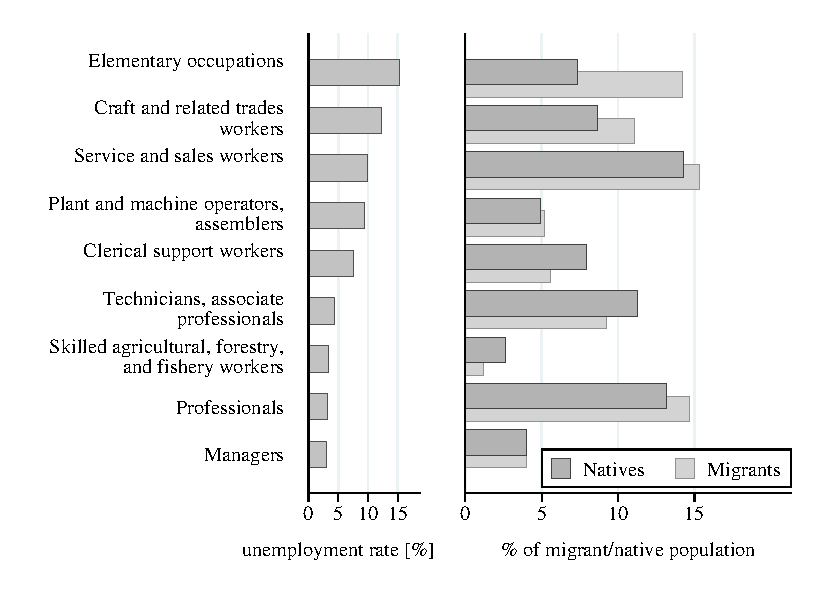
\includegraphics[scale=0.85]{figure_bar.pdf}
  \caption{Ukázka sloupcového grafu, který neurazí. Převzato z~\citet{Tepperova2017}.}
  \label{fig:bar}
\end{figure}

\subsection*{Literatura a zdroje dat}

\begin{itemize}[itemsep=2pt, topsep=2pt]
  \item Doporučuji odkazy ve jmenném formátu, např.\ „(Wooldridge, 2020)“, ne číslem, např.\ „[3]“.
  \item Rozlišujte textovou a parentetickou citaci: „Novák (2019) podstatně rozšířil výsledky publikované v~(Dvořák a Krásná, 2010; Adamská, 2013).“
  \item Seznam literatury patří na konec práce, ne do poznámek pod čarou. Musí mít jednotný formát (ideálně některý ze standardních, např.\ APA, nekombinovat) a reference jsou seřazené abecedně.
  \item Napsat, že data pocházejí ze serveru kaggle.com, nestačí! Citujte přesný datový soubor a uveďte ho v~seznamu zdrojů. Ideálně zjistěte co nejvíc o~původu dat (kdo je sbíral, jak a kdy), abyste mohli čtenáři poskytnout úplný obrázek.
\end{itemize}

\subsection*{Rozsah}

Zkušenost praví, že práce s~rozsahem do čtyř stran mají vyšší průměrné hodnocení než práce na pět a více stran. Jednoduše proto, že dlouhé práce zpravidla obsahují balast, který do nich nepatří: malou tabulku pro každý statistický test, opakované zápisy nulových hypotéz, korelační matici rozprostřenou do tří špatně naformátovaných tabulek apod.

\begin{thebibliography}{9}
\bibitem[Angrist a Pischke(2009)]{Angrist2009} Angrist, J. D., \& Pischke, J.-S. (2009). \textit{Mostly harmless econometrics: An empiricist's companion}. Princeton University Press.

\bibitem[Lukeš a kol.(2013)]{Lukes2013} Lukeš, M., Zouhar, J., Jakl, M., \& Očko, P. (2013). Faktory ovlivňující vstup do podnikání: začínající podnikatelé v~České republice. \textit{Politická ekonomie}, \textit{61}(2), 229--247.

\bibitem[Tepperová a kol.(2017)]{Tepperova2017} Tepperová, J., Zouhar, J., \& Wilksch, F. (2017). Intra-EU migration: Legal and economic view on jobseekers' welfare rights. \textit{Journal of International Migration and Integration}, \textit{18}(3), 917--936. \url{https://doi.org/10.1007/s12134-016-0509-6}
\end{thebibliography}

\end{document}
